\documentclass[letter,portrait]{article}

\usepackage{amsmath,amssymb}

\usepackage[dvipsnames]{xcolor}

\usepackage{listings}
\lstset{language=}
\renewcommand\lstlistingname{File}
\renewcommand\lstlistlistingname{Files}
\lstset{numbers=none, numberstyle=\tiny, stepnumber=1, numbersep=5pt,captionpos=b,frame=single,breaklines=true,basicstyle=\small, tabsize=4}

\usepackage{graphicx,color,epsfig}

	
\usepackage[format=plain,indention=.5cm,margin=10pt,font={small,singlespacing}]{caption}%custom captions.
\usepackage{parskip}

	
	
\usepackage{enumitem}


%for inputting bertini real input files
\newcommand{\Filenobox}[3]{

\lstinputlisting[frame=none,
	breaklines=true,
	caption={#1},
	label=#2]{#3}

}

\usepackage{marginnote}
\renewcommand*{\marginfont}{\color{red}\sffamily\tiny}
\newcommand{\sidenote}[1]{\textcolor{red}{$\star$}\marginnote{#1}}


\usepackage[utf8]{inputenc}
\usepackage{multirow, bigstrut, booktabs}
\usepackage{longtable}
\usepackage{tabu}



\usepackage{fancyhdr}

\fancypagestyle{front}{

    	\fancyhf{} % sets both header and footer to nothing
		\renewcommand{\headrulewidth}{0pt}

       \fancyfoot[RO, LE]{\thepage} %Page Number
       \fancyfoot[C]{} 
}


\fancypagestyle{main}{
    	\fancyhf{} % sets both header and footer to nothing
		\renewcommand{\headrulewidth}{0pt}

       \fancyfoot[RO, LE]{\thepage} %Page Number
       \fancyfoot[C]{} 

       \fancyhead[LE,RO]{\leftmark}
       \fancyhead[LO,RE]{\rightmark}
}

\usepackage{authblk}


% hyperref must be last
\usepackage[colorlinks]{hyperref}
\hypersetup{
    colorlinks=true,       % false: boxed links; true: colored links
    linkcolor=Plum,          % color of internal links (change box color with linkbordercolor)
    citecolor=violet,        % color of links to bibliography
    filecolor=magenta,      % color of file links
    urlcolor=blue           % color of external links
}




\title{Real answers to complex questions with numerical nonlinear algebra}
\author{Danielle Amethyst Brake $^1$} %  and Jonathan Hauenstein $^2$


\date{$^1$ University of Wisconsin - Eau Claire \\[\baselineskip] \today} % \\ $^2$ University of Notre Dame

\newcommand{\C}{\mathbb{C}}
\newcommand{\R}{\mathbb{R}}
\newcommand{\1}{{\tt \_1}}
\newcommand{\2}{{\tt \_2}}

\newcommand{\tools}[1]{{\em suggested tools:} {\tt #1}}

\begin{document}


\maketitle
\thispagestyle{empty}
\vfill
\begin{center}
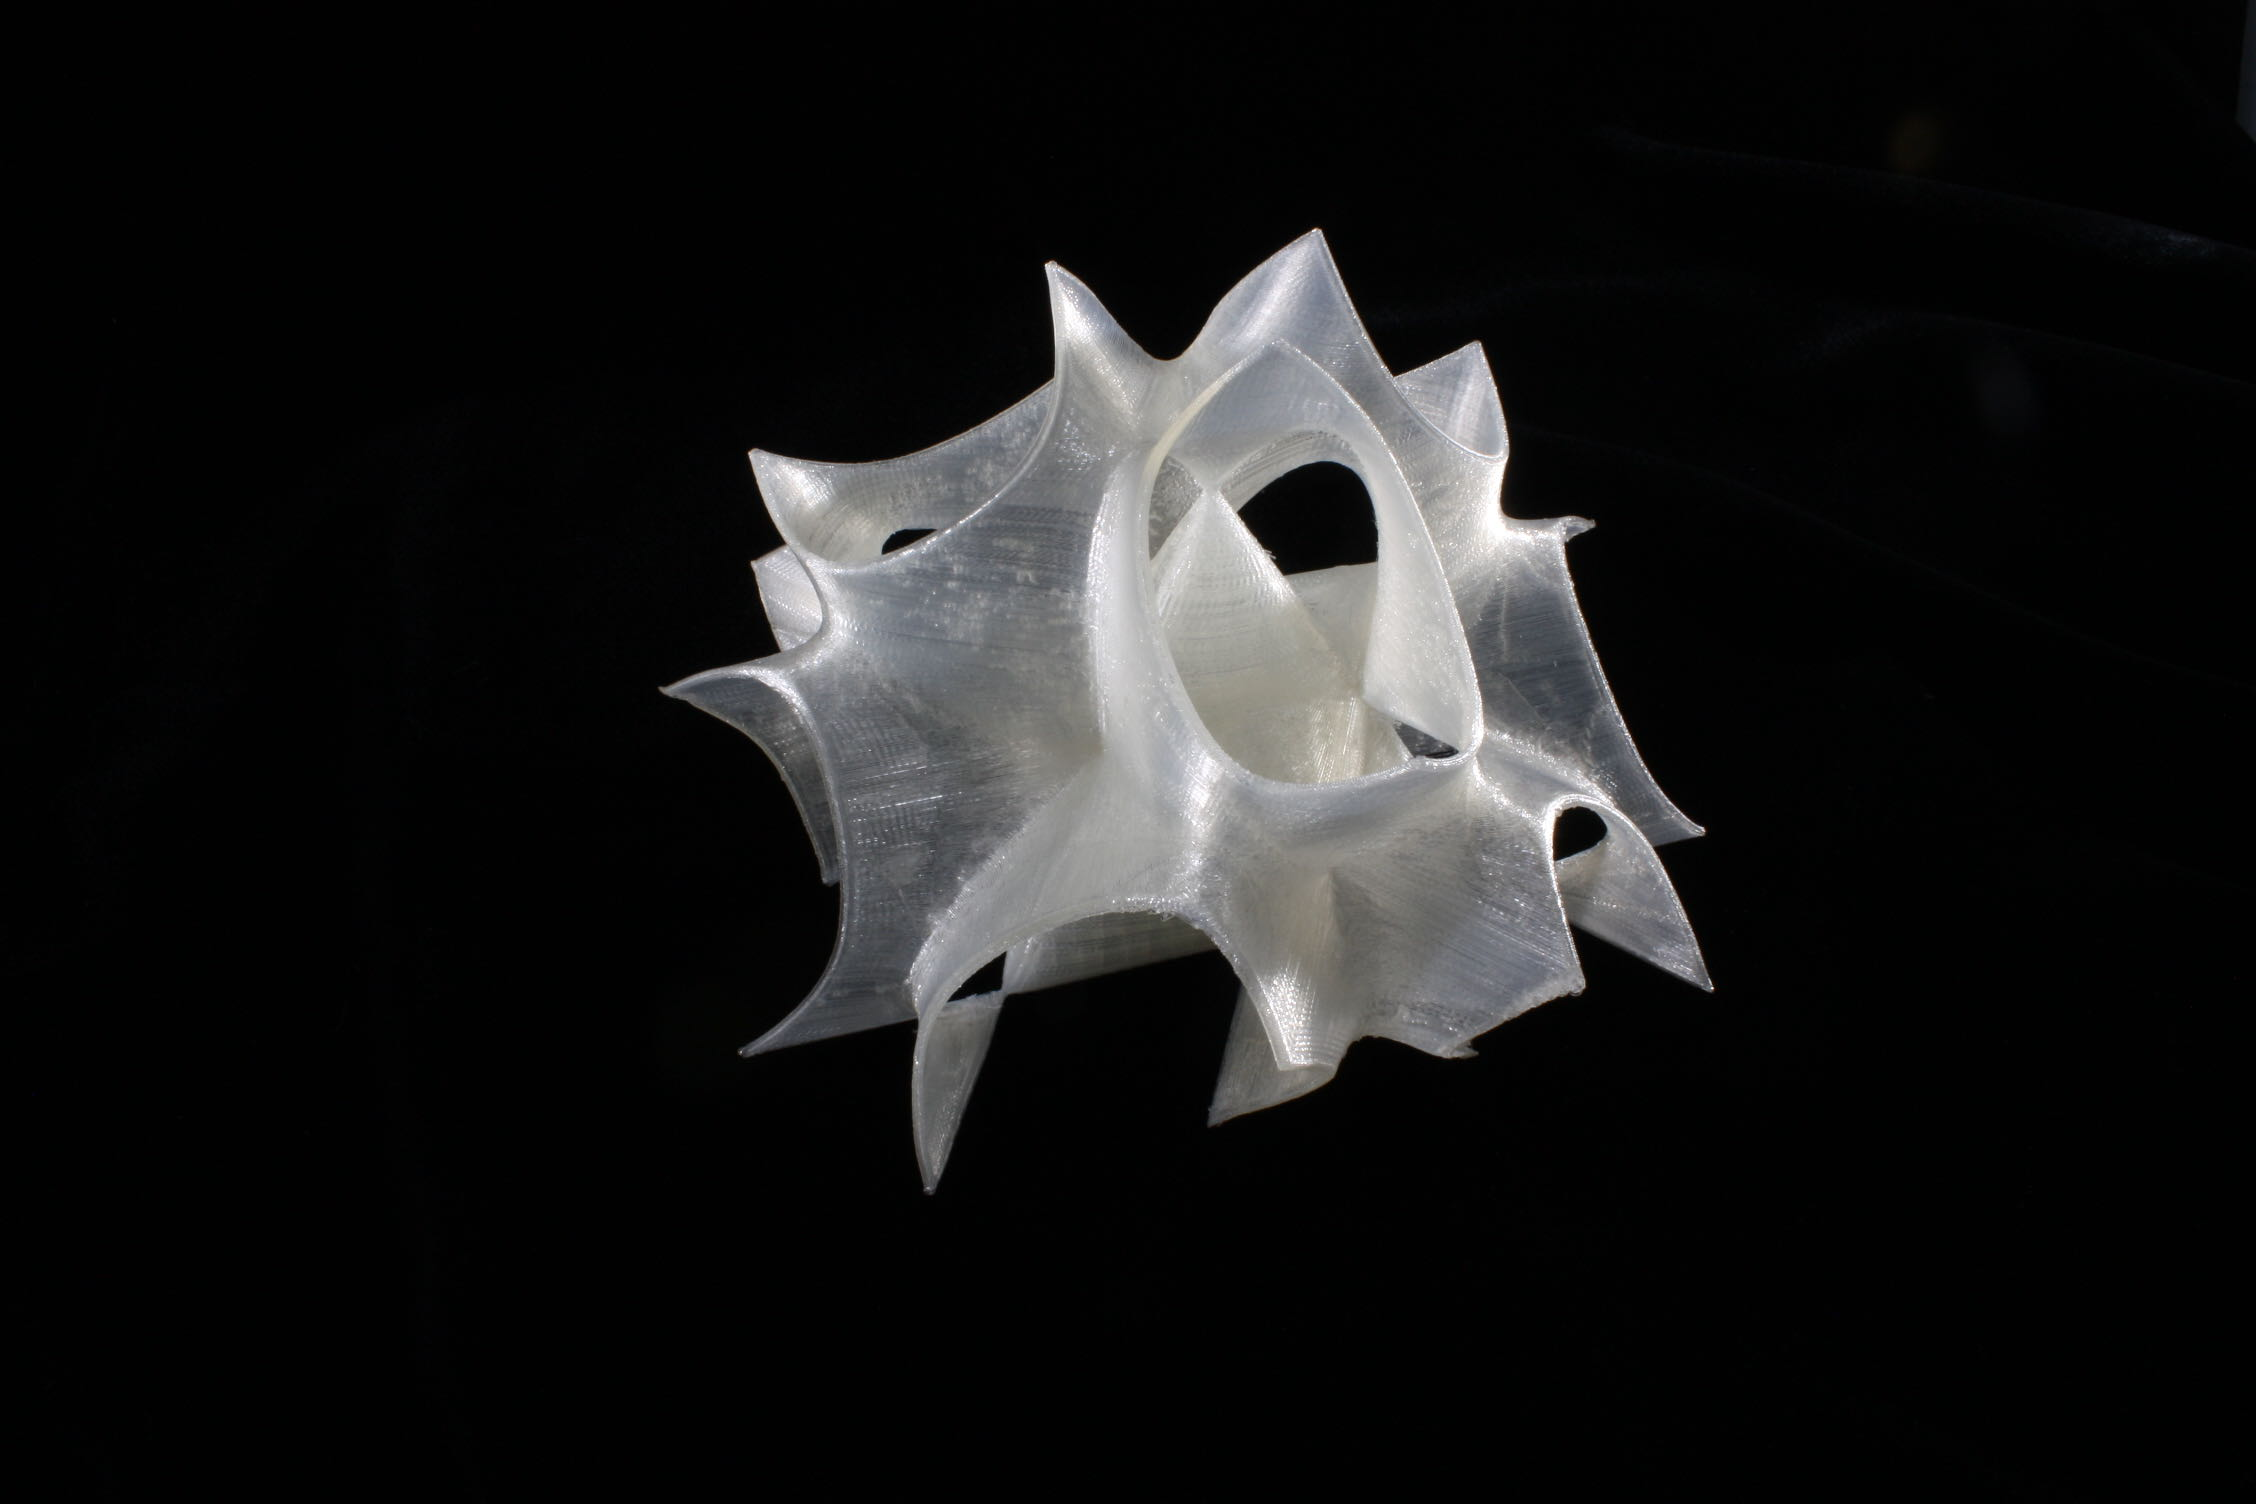
\includegraphics[width=3in]{diagrams/ICERM_surface_printed.jpg}
\end{center}
\vfill
\clearpage


\pagestyle{plain} 
  \pagenumbering{roman} 
  \setcounter{page}{1}

\tableofcontents
  \eject
  \pagenumbering{arabic} 
  \setcounter{page}{1}
  \eject

\clearpage


\section{Preface}

\subsection{A note from an author}
The motivation for this guide is the \href{https://icerm.brown.edu/programs/sp-f18/w4/}{Nonlinear Algebra Bootcamp}, at \href{https://icerm.brown.edu/programs/sp-f18/}{the workshop on Nonlinear Algebra}  at \href{https://icerm.brown.edu/}{the International Center for Experimental Research in Mathematics} at Brown University, Fall 2018.  

These exercises are meant to help train you to use tools in the world of {\em real} computational nonlinear algebra.  They were prepared by a numerically aligned person, so they have that flavor to them.  This document does not contain a full set of references, though they are in some places provided.  Feedback is welcomed to \href{mailto:danielleamethystbrake@gmail.com}{danielleamethystbrake@gmail.com}.

We'll start by solving a few simple problems, and build up to some that are deeper.  The challenge problems toward the end are open, credited to the researcher who posed it.  They're food for thought and intended as the beginning of ongoing conversations with people here at ICERM this semester.  

I hope these problems spur you forward! $\heartsuit$

\subsection{Tools}

There are lots of tools in the belt of a computational or applied nonlinear algebraist.  Here are some, in $\alpha\beta$ order:

\begin{itemize}
\item Alpha certified. command-line.
\item Bertini and its friends.
		\begin{itemize}
			\item Bertini -- command-line.  Text files as input and output.  Interfaces through other languages, including Macaulay2, Matlab,\footnote{From Danielle: if you want to use Matlab for interfacing with Bertini, check out ({\tt git clone}, ha) my mediocrely documented repo of Bertini1 utilities at \url{https://github.com/ofloveandhate/brakelab}.} and others.  
	\item Bertini\_real -- command-line, visualization in Matlab and Python
	\item Paramotopy -- command line, visualization in Matlab
	\item Bertini2 -- command line, Python.  experimental
		\end{itemize}
\item CoCoa -- command line
\item Hom4PS -- command line
\item \href{https://www.juliahomotopycontinuation.org}{homotopycontinuation.jl}
\item Macaulay2 -- command line, $\exists$ an online interface.
\item Mathematica -- proprietary, decent symbolics.  Sideways cursors.\footnote{Pardon the editorializing.  I {\em am} the author, tho.  I think I get to do that.}
\item Maple -- proprietary, good symbolics.  Not Danielle's favorite for numerics.
\item Matlab -- proprietary, oriented well to arrays of numbers.  Weaker symbolics.
\item PHCPack -- command line, online interface

\end{itemize}


If you want Bertini-flavored input files for any of the Herwig Hauser surfaces, many of them are available at the {\tt test/surface/name} folder in the GitHub repo for Bertini\_real.

If you have issues or questions or suggestions, there are many software authors here in the building this semester, so ask around, they're sure to help you!



\subsection{Notation}

Here are some notes on notation used in this training guide

\begin{itemize}
\item	I will horrify you with my abuses of notation.  Things are vectors when they are, and aren't when they aren't.  $x$ is multiple things in one line of math.  Yep.  This'll get cleaned up over time, as I hope this little booklet, which is mostly just formatting right now, turns into something bigger.
\item $\square$ -- a placeholder.  I also like \1 and \2 (those come from C++).
\item When in doubt, the system equals zero.  Don't make me write $=0$ all over the place.
\end{itemize}

\subsection{Acknowledgements}

In the preparation of this training guide, I had help from many colleagues, including: Jon Hauenstein, Elizabeth Gross, Jeff Sommars, and Anton Leykin.









% ________             _____       _____                
% ___  __/____________ ___(_)_________(_)_____________ _
% __  /  __  ___/  __ `/_  /__  __ \_  /__  __ \_  __ `/
% _  /   _  /   / /_/ /_  / _  / / /  / _  / / /  /_/ / 
% /_/    /_/    \__,_/ /_/  /_/ /_//_/  /_/ /_/_\__, /  
%                                              /____/   



\clearpage
\section{Training exercises}

These should be solvable using off-the-shelf software.  


\subsection{Basic}

\subsubsection{A simple quadratic}
\label{sec:1x1}

Use as many packages for numerical nonlinear algebra as you can to find the real roots of
\[
f(x) = 
x^2-2
\]
where in this case we mean, find the $x$ such that $f(x) = 0$.  


\subsubsection{A simple 2x2 system}
\label{sec:2x2}


Use many numerical softwares for nonlinear algebra to find the real roots of
\[
f(x) = \begin{bmatrix}
x^3 + xy - 3y \\ 
xy - 3x^5 + \sqrt{2}
\end{bmatrix}
\]

\subsubsection{A 4x4 system}
\label{sec:3x3}

Describe the real solution set of
\marginnote{}
\[
\begin{bmatrix}
(x^2+y^2)^3-4x^2y^2(z^2+1) \\ %eistute
x^4-2.5x^2y^3 -xz^3 +y^6 -y^2z^3 \\ %seepferdchen
4(\phi^2x^2-y^2)(\phi^2y^2-z^2)(\phi^2z^2-x^2) - (1+2\phi)(x^2+y^2+z^2-w^2)^2w^2 \\ % the barth sextic
w-1
\end{bmatrix}
\]
where $\phi$ is the golden number.

What happens as you vary the affine patch -- that is, vary the last equation to be another linear function of the variables?




\subsection{Intermediate}

\subsubsection{Roots of cyclic polynomials}
\label{sec:cyclic}


% \marginnote{needs definition of cyclic poly}



Compute the roots of the cyclic-$n$ polynomials,\footnote{See \cite{dai2003computing} for a description of the cyclic-$n$ system.  Python code to generate the system in a given set of variables is in Appendix~\ref{app:cyclic}} for $n \in \{1, \ldots, m\}$ for some practical $m$.  How many are real?  




% take a curve, set up Lagrange multiplier method to find critical points, build a complex equivalent to the curve, etc.








% \subsubsection{*The complex numbers as two copies of the reals}

% Express a system where we want reality from the real and imaginary components, and couple them with $x+iy$

% Example -- Riemann surfaces


% \subsubsection{*Isotropic coordinates}
% \label{sec:isotropic}

% Express a system where the real and imaginary are bound together by angle and magnitude rather than real and imaginary

\subsubsection{Certification}
\label{sec:certification}

Certify the reality of the solutions from \ref{sec:1x1}, \ref{sec:2x2}, \ref{sec:3x3}, \ref{sec:cyclic}.

% \tools{alpha certified}








% \subsubsection{*Something about the twisted cubic}

% The twisted cubic is a fabulous space curve.  




\subsubsection{Basic surface plotting}
\label{sec:basic_surface_plot}

Make a picture of the Cayley Cubic.

What happens in your plot if you center your view tightly around one of the singularities?  Do the connected components actually join?  At a {\em point}?  How far in can you zoom?  What if you change settings?  Label the singularity in-figure, and save your picture to disk at ready-to-publish quality.



\subsubsection{Varying components on parameters}

Describe the way the real components of an elliptic curve depend on its parameters.





%  ___                                                   
% (  _`\                                                 
% | | ) |   __     __   _ _      __   _ __               
% | | | ) /'__`\ /'__`\( '_`\  /'__`\( '__)              
% | |_) |(  ___/(  ___/| (_) )(  ___/| |                 
% (____/'`\____)`\____)| ,__/'`\____)(_)                 
%                      | |                               
%                      (_)                               
%                     _      _                           
%                    ( )    (_ )                         
%  _ _    _ __   _   | |_    | |    __    ___ ___    ___ 
% ( '_`\ ( '__)/'_`\ | '_`\  | |  /'__`\/' _ ` _ `\/',__)
% | (_) )| |  ( (_) )| |_) ) | | (  ___/| ( ) ( ) |\__, \
% | ,__/'(_)  `\___/'(_,__/'(___)`\____)(_) (_) (_)(____/
% | |                                                    
% (_)                                                    

\clearpage
\section{Deeper problems}


% \subsection{Optimization}
% \subsubsection{*A raw optimation problem}

% In this problem, we are interested in finding the minimum value of . The solutions {\em are} the optima, so when the software returns solutions, we are essentially done.


% \subsubsection{*What's the optimal solution?}

% The solutions must be post-processed to compute the optima.





% \subsubsection{*Is there a parameter point such that \1? part 1}

% \tools{
% \begin{itemize}
%   \item Bertini, PHCPack, Hom4PS, Macaulay2 NumericalAlgebraicGeometry
%   \item Paramotopy
% \end{itemize}
% }
% Here's a typical problem: we have a parameterized polynomial system, and we want to find out whether there is a parameter point such that \_1.  That is, \_1 is a placeholder for your favorite property, and you want to find a place in the parameter space such that your property is satisfied.

% Let's specify \1 to be ``All solutions to the parameter point lie outside the unit cube''.  

% \[
% f = \begin{bmatrix}
% a
% \end{bmatrix}
% \]

% I was thinking of this problem being one of post-processing, so you would solve the problem using the tool of your choice, and then filter the solutions in a related tool.  I'd use Bertini and Matlab.  You do you.






\subsection{Positive dimension}



% \subsubsection{*Is there a real point on a given component?}

% This problem investigates a kinematic design problem where the solution space is positive dimensional.  We want to find out whether there is a real solution on this algebraic variety.








\subsubsection{A real point on every connected component}

% Now, let's look at things a little differently.  Consider the following implicitly given quartic real plane curve from \cite{brake2016computing} (\url{https://arxiv.org/abs/1605.04203}):

% \[x^4 + y^4 - (x - y)^2 (x + y) = 0 \label{eqn:butterfly}\]

% One common question asked in the real realm is {\em are there any real points?}, without necessarily caring how many, or what the dimension of the real set is.  A full reference for what we're about to do is ``Numerically computing real points on algebraic sets''  \cite{hauenstein2013numerically}.  A less theoretically focused perspective is given in \cite{bates2013numerically} section 14.5.

% Here's a brief explanation and demonstration, through which you will be guided.  The crux of the method is to compute critical points of the function measuring distance between the complex component and a random real point.  Randomly complexly perturbating the system $f$ and taking the perturbation to zero while homotoping a random complex point to the chosen real point guarantees a real point on each connected component.

% Choose a random real point, and call it $a$.  Since our ambient space is $\R^2$, we need two random coordinates.  Generate a random {\em real} $a$ using  your favorite RNG.  Next we take the $d$, distance function between an unspecified point $(x,y)$ and $a$.   

% \[
% D = \sqrt{(x-a_1)^2 - (y-a_2)^2}
% \]
% but because it's easier and equivalent to just deal with distance-squared, we'll just do that.  
% \[
% d = (x-a_1)^2 - (y-a_2)^2
% \]

% \[
% \begin{bmatrix}
% x-a & \nabla f_1(x)^\intercal & ... & \nabla f_N(x)^\intercal
% \end{bmatrix}
% \]


Compute at least one point on every real connected component of the octic from the paper ``A projective surface of degree eight with 168 nodes" \cite{endrass1995projective}.%
\footnote{A Bertini input file for a particular patching of it may be found at {\tt test/surface/dihedral} at Danielle's GitHub repo for Bertini\_real.}
How do you deal with the projectivity? 

Certify the reality of your solutions.

Challenge: Code the method generically so that you may apply it to any component of any variety with one function call.  Document it.






\subsubsection{Are there completely naked singularities?}

Surfaces often have singularities, and sometimes those singularities are naked -- not surrounded in a full-dimension sense by the surface, but instead the local dimension in a neighborhood of some point is 1 or 0, rather than 2.

Consider 
\begin{itemize}
\item the Whitney Umbrella:

\[
x^2 - y^2z
\]

\item Buggle:
\[
x^4y^2+y^4x^2-x^2y^2 + z^6
\]
\end{itemize}


Determine if they have any naked singularities.  Deflate the singularities.  Are there any singularities on these singularities?  If so, deflate them, all the way, so that for every singularity, you have a polynomial system with that singularity as a regular point.  Describe the resulting polynomial systems.







\subsubsection{An algebraic version of a M\"obius strip}

We can generate a torus as a surface of revolution with a circle offset from the origin -- hey, we've all taken Calc 1.  We can generate a flattened torus -- a donut with insufficient leavening -- by using an ellipse.  We can generate a twisty donut by revolving the ellipse about its center one full revolution as the torus is spun about the $z$-axis.  It looks like a M\"obius strip, but is definitely not a M\"obius strip, so let's call it an algebraic M\"obius-like surface.  

\begin{center}
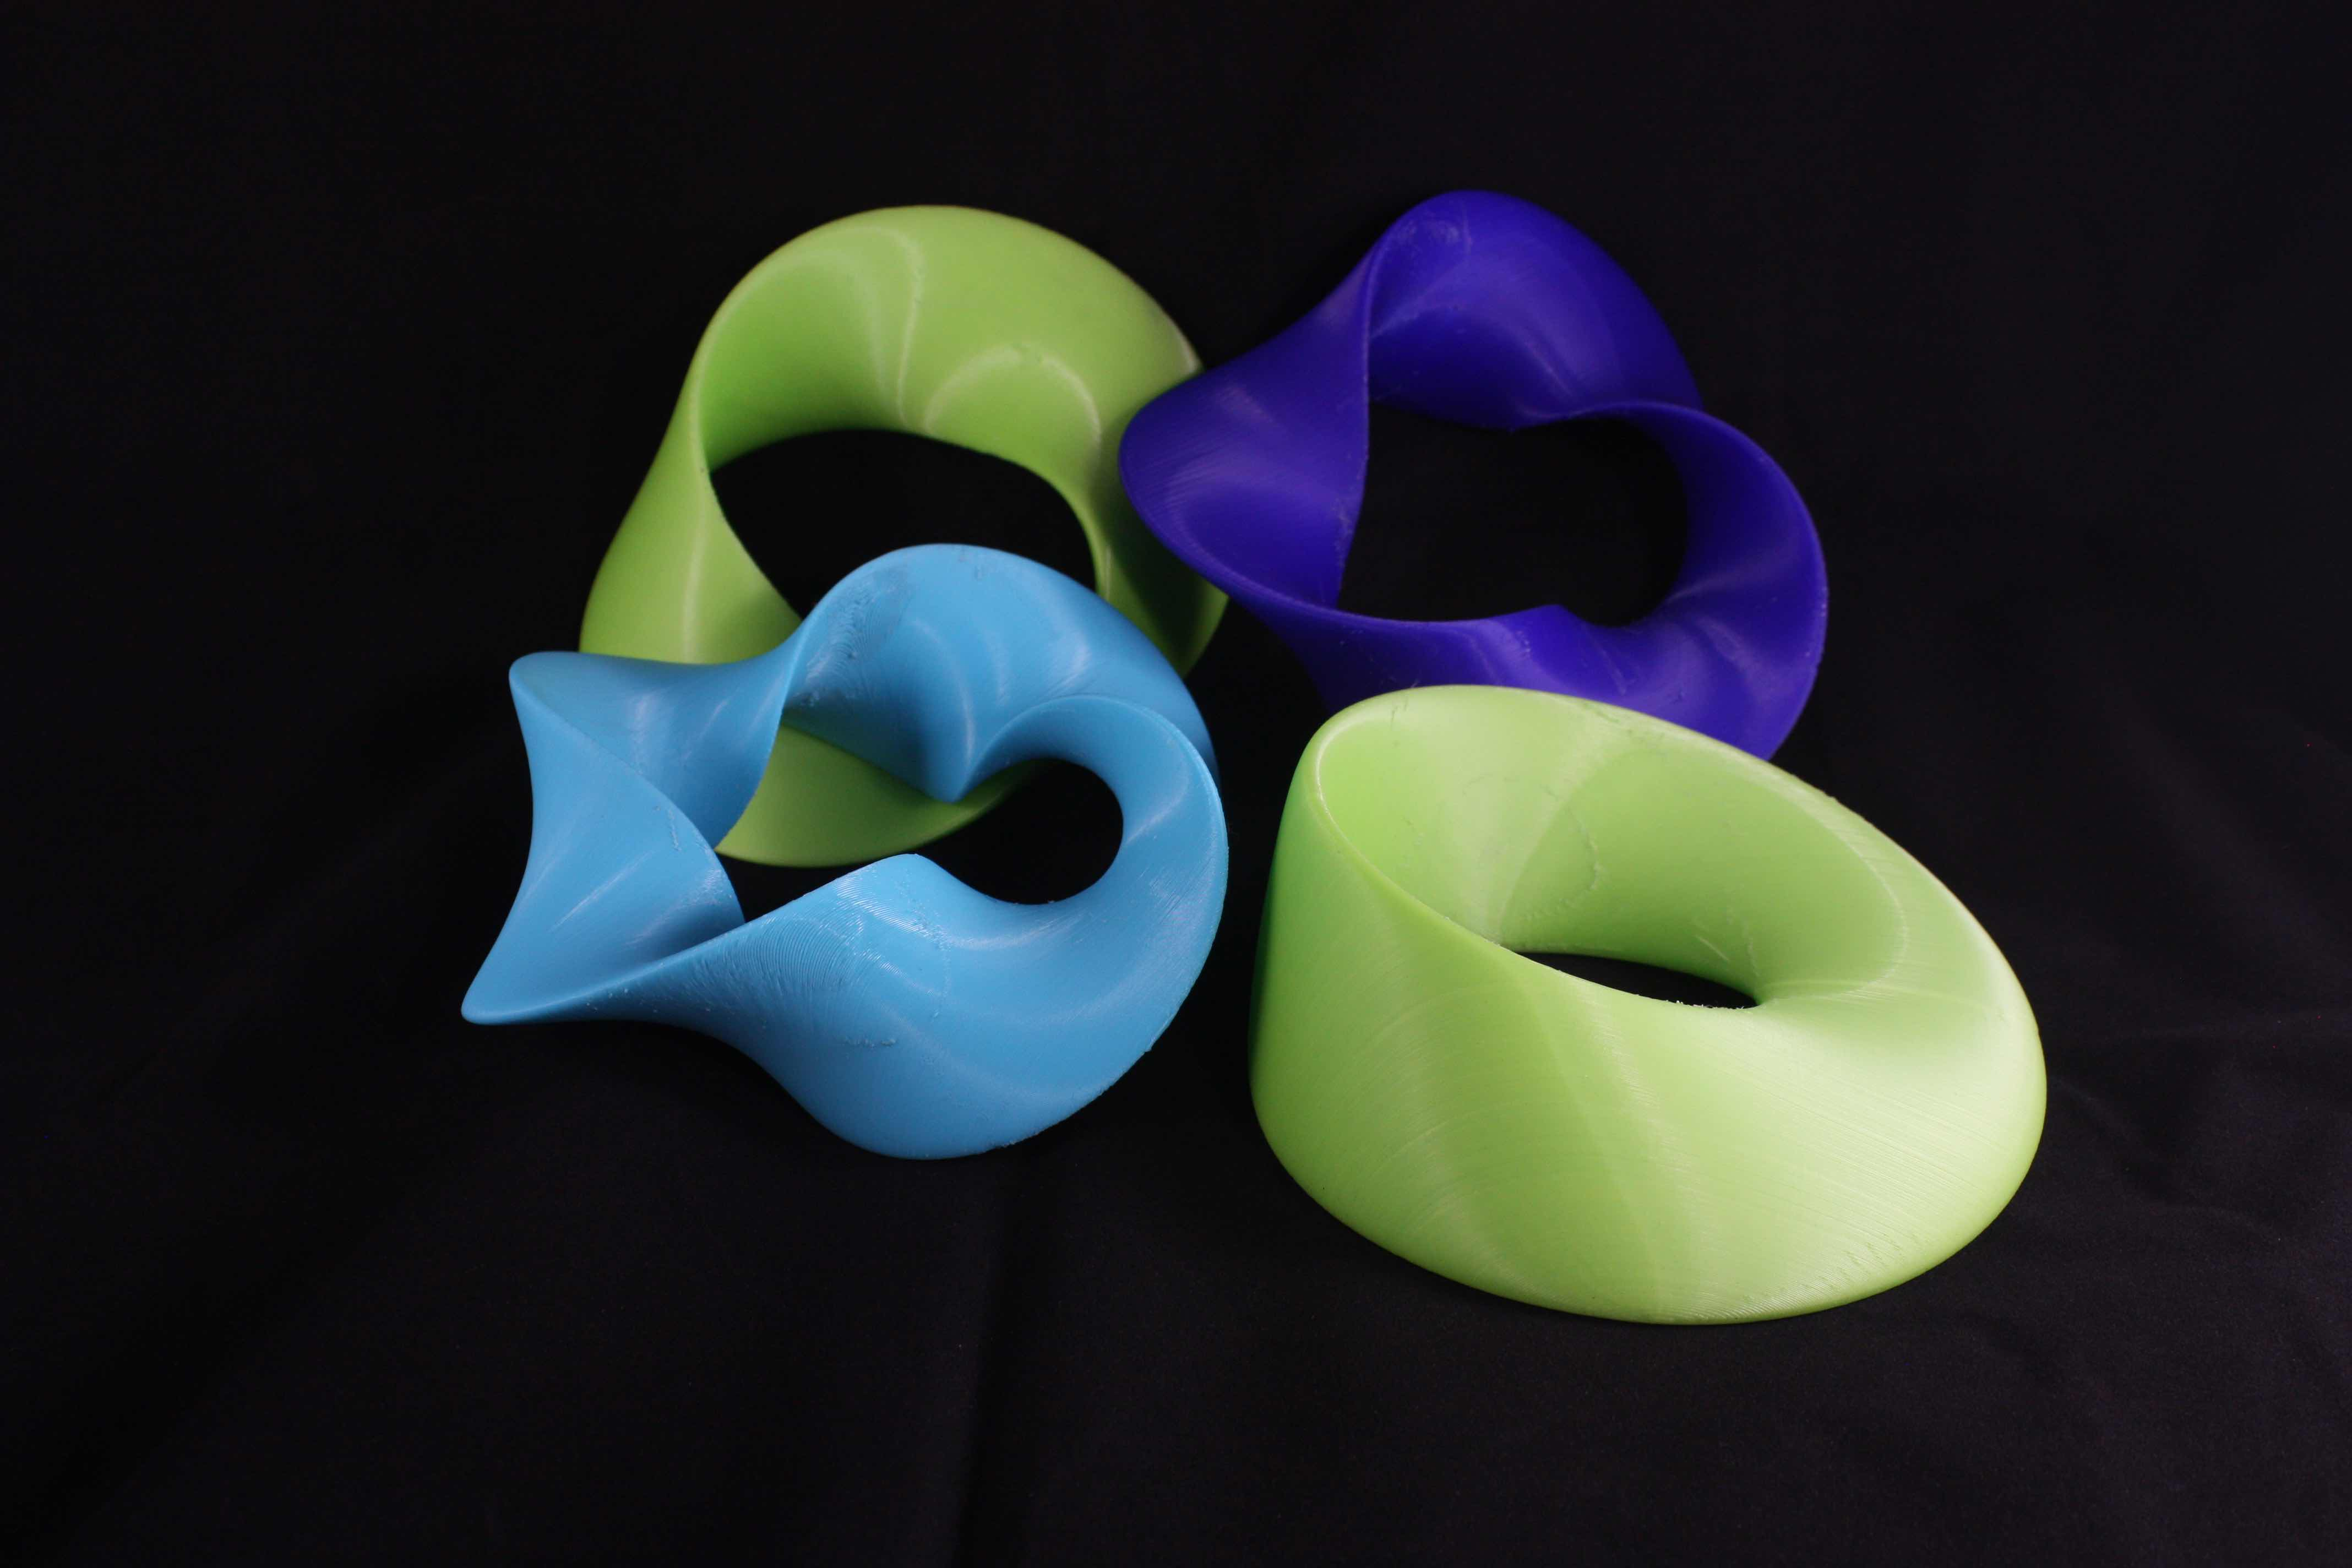
\includegraphics[width=3in]{diagrams/mobius.jpg}
\end{center}

Is such a M\"obius-like surface smooth?  What happens in your rendering software if you make the number of twists very large?

















 %   ____ _           _ _                            
 %  / ___| |__   __ _| | | ___ _ __   __ _  ___  ___ 
 % | |   | '_ \ / _` | | |/ _ \ '_ \ / _` |/ _ \/ __|
 % | |___| | | | (_| | | |  __/ | | | (_| |  __/\__ \
 %  \____|_| |_|\__,_|_|_|\___|_| |_|\__, |\___||___/
 %                                   |___/           



\clearpage
\section{Challenges and open problems}

These problems are written in the first person, in the perspective of the credited mathematician.



\subsection{Find a parameter point such that \1?}

$\star$ From \href{https://math.hawaii.edu/wordpress/people/egross/}{Elizabeth Gross} $\star$


This paper (\url{https://arxiv.org/pdf/1502.03188.pdf}) focuses on a single parameterized polynomial system arising from a particular signaling pathway model.  We know that we can find parameters that give rise to 0, 1, 2, and 3 real positive solutions.  We like to challenge people to see if they can find a set of parameters that give rise to more than 3 real positive solutions (See Remark 4.2 in the paper)--so far nobody has been able to.~\footnote{aside from Danielle: I would use Paramotopy's search function to do this...}

If people want to experiment with it, the network is one of the pre-loaded examples in the ReactionNetworks.m2 package (\url{http://www2.macaulay2.com/Macaulay2/doc/Macaulay2-1.11/share/doc/Macaulay2/ReactionNetworks/html/_wnt.html}).






\subsection{Find the posreal solutions}

$\star$ From \href{http://homepages.math.uic.edu/~sommars/}{Jeff Sommars} $\star$

I was contacted by a quantum physics grad student in Sydney who was trying to find positive real solutions to several sets of polynomial systems (I expect they were a parametrizable family, but I couldn't get him to give me a generalized version). I've pasted in the simplest one below in Macaulay2 format. It's a 16x16 system, but the other ones he was interested in were more like 30x30...

\begin{verbatim}
R = CC[a1,a2,a3,a4,b1,b2,b3,b4,c1,c2,c3,c4,k41,k12,k23,k34]
polys = {b1^2 + 0.2*a1*c1 + c1^2 + a1^2*k41 - a4^2*k41
  , a1*b1*(-0.5 + k41) - a4*b4*k41
  , b2^2 + 0.2*a2*c2 + c2^2 - a1^2*k12 + a2^2*k12
  , a2*b2*(-0.5 + k12) - a1*b1*k12
  , b3^2 + 0.2*a3*c3 + c3^2 - a2^2*k23 + a3^2*k23
  , a3*b3*(-0.5 + k23) - a2*b2*k23
  , b4^2 + 0.2*a4*c4 + c4^2 - a3^2*k34 + a4^2*k34
  , a4*b4*(-0.5 + k34) - a3*b3*k34
  , -1 + a1^2 + b1^2 + c1^2
  , -1 + a2^2 + b2^2 + c2^2
  , -1 + a3^2 + b3^2 + c3^2
  , -1 + a4^2 + b4^2 + c4^2
  , 0.1*a1^2 - 0.1*b1^2 - 0.1*c1^2 - 1.*a1*c1*(-0.5 + k41) + a4*c4*k41
  , 0.1*a2^2 - 0.1*b2^2 - 0.1*c2^2 - 1.*a2*c2*(-0.5 + k12) + a1*c1*k12
  , 0.1*a3^2 - 0.1*b3^2 - 0.1*c3^2 - 1.*a3*c3*(-0.5 + k23) + a2*c2*k23
  , 0.1*a4^2 - 0.1*b4^2 - 0.1*c4^2 - 1.*a4*c4*(-0.5 + k34) + a3*c3*k34}

\end{verbatim}

This is probably out of reach of the {\tt fall18} server.  Can you use resources at your home institution?  Write to Jeff for the 30x30 system.


\subsubsection{How many edges?}


$\star$ from \href{https://danielleamethyst.org}{Danielle Brake} $\star$



In a curve decomposition, we break the curve $\mathcal{C}$ into cells called {\bf edges}.  A circle always decomposes into two edges -- and we get a square.  
\begin{itemize}
\item What are all possible numbers of edges that a cellular decomposition of some $\mathcal{C}$ may have (depending on the projection used)? 
\item Is it possible to get other regular polygons, with or without edge-merging?  Construct a general method.
\end{itemize}




\subsubsection{Regular polyhedra as raw cellular decompositions}


$\star$ from \href{https://danielleamethyst.org}{Danielle Brake} $\star$

In a surface decomposition, we break the surface $\mathcal{S}$ into cells called {\bf faces}.  When you decompose a sphere, you always get a regular octohedron -- neat!  Which of the other Platonic Solids can be achieved as a numerical cell decomposition of some $\mathcal{S}$?  



% \subsection{Local real decomposition}

% $\star$ from \href{https://danielleamethyst.org}{Danielle Brake} $\star$


% Give the local {\em real} decomposition, about the origin, of the Wigwam surface
% \[
% x^2+y^2z^3
% \]





% \subsection{*Critical sets through detjac and nullspace}

% $\star$ from \href{https://danielleamethyst.org}{Danielle Brake} $\star$

% I want to know: is there a better way to compute critical sets of critical sets?

% Let me describe my current method.  But first, I need to explain a bit about the decomposition routine implemented in Bertini\_real.  

% Bertini\_real impements the implicit function theorem, which says that away from a set of measure zero, an object of dimension $k$ can be parameterized by $k$ parameters.  On the set of measure zero, though, it takes fewer parameters,  This set is called the {\em critical set} of the decomposition.  

% The critical set depends on the method being used to assign $k$ parameters to points with $n$ coordinates -- in the case of Bertini\_real, the coefficients of the linear projection $\pi$ being used.  Here's how I compute it:

% Your square system $f$ which defines the surface.  Take it's Jacobian.  Take the Jacobian of the projection (it's a linear projection onto two coordinates, to it's a constant 2x$N$ matrix).  Vertically concatenate them.  Take the determinant $D$. Then $f\prime = [f D]=0$ gives the critical curve.

% Now you need to compute the critical points on the critical curve.  Do the same thing. Take $J(f\prime)$, concatenate on the botton the matrix for the first line of $\pi$, take the determinant ($D\prime)$, set it equal to zero.  This,  $f\prime\prime = [f D D\prime] = 0$ gives the critical points of the critical curve of the surface with respect to $\pi$.  

% Now, I know that determinants are ... challenging.  So, whatever the tail end of the 

% Is there a better way?










%                             .-') _  
%                            ( OO ) ) 
%    ,------.,--. ,--.   ,--./ ,--,'  
% ('-| _.---'|  | |  |   |   \ |  |\  
% (OO|(_\    |  | | .-') |    \|  | ) 
% /  |  '--. |  |_|( OO )|  .     |/  
% \_)|  .--' |  | | `-' /|  |\    |   
%   \|  |_) ('  '-'(_.-' |  | \   |   
%    `--'     `-----'    `--'  `--'   

\clearpage
\section{Just for fun}

\subsection{3d printing}

\subsubsection{Obtain an STL}
\label{sec:stl}
A {\tt .stl} file, which defines a 3-dimensional triangulation, is 3d printable if there is a well-defined and water-tight interior, as determined by the face normals.
Obtain a 3d-printable {\tt .stl} file for 

\begin{itemize}
\item 
the surface Leopold:
\[
x^2y^2z^2+3x^2+3y^2+z^2-1 
\] 
\item the Whitney Umbrella
\[
x^2 - y^2z
\]
How do you deal with the handle?
\item 
the ICERM surface from Cynthia's problem set:\footnote{coefficients here are negated, and the 8 was dropped}
\begin{align*}
f = &3x^2 - x^2y^4 - x^4y^2 - 2x^2z^2 - x^2z^4 - x^4z^2 - 2y^2z^2 - y^2z^4 - \\
&y^4z^2 - 2x^2y^2 - 3x^4 + x^6 + 3y^2 - 3y^4 + y^6 + 3z^2 - 3z^4 + z^6 + 10x^2y^2z^2 - 1
\end{align*}
bounded inside $[-2,\,2]^3$ and below the plane $x+y+z=1.1$.

\item The 4-dimensional surface given by
\begin{align*}
f_1 &= w^2 + x^2 + y^2 + z^2 - 1 \\
f_2 &= 2wyz - x(y^2 + z^2)
\end{align*}

\end{itemize}
























%  _______  _______  _______  _______  _        ______  _________         
% (  ___  )(  ____ )(  ____ )(  ____ \( (    /|(  __  \ \__   __/|\     /|
% | (   ) || (    )|| (    )|| (    \/|  \  ( || (  \  )   ) (   ( \   / )
% | (___) || (____)|| (____)|| (__    |   \ | || |   ) |   | |    \ (_) / 
% |  ___  ||  _____)|  _____)|  __)   | (\ \) || |   | |   | |     ) _ (  
% | (   ) || (      | (      | (      | | \   || |   ) |   | |    / ( ) \ 
% | )   ( || )      | )      | (____/\| )  \  || (__/  )___) (___( /   \ )
% |/     \||/       |/       (_______/|/    )_)(______/ \_______/|/     \|
                                                                        

\appendix
\clearpage
\section{Code}
\subsection{Cyclic}

PyBertini code generating the cyclic-$n$ polynomials

\label{app:cyclic}
\begin{verbatim}
def cyclic(vars):
    n = len(vars)
    f = [None] * len(vars) # preallocate
    y = [] #make a circle of variables.  there are more elegant ways to do this
    for ii in range(2):
        for x in vars:
            y.append(x)

    # use a product of a list comprehension to construct the n-1 functions
    for ii in range(n-1):
        f[ii] = numpy.sum( [numpy.prod(y[jj:jj+ii+1]) for jj in range(n)] )

    # the last function is the product of all the variables, minus one
    f[-1] = numpy.prod(vars)-1
    return f

\end{verbatim}









\clearpage









\bibliographystyle{plain}
\bibliography{real_nonlinear.bib}




\end{document}



